\documentclass[tikz,border=1pt]{standalone}
\usepackage[libertine]{newtxmath}\usepackage{libertine}
\usetikzlibrary{positioning,arrows.meta}
\newcommand{\dodo}[1]{\mathrm{do}(#1)}
\begin{document}
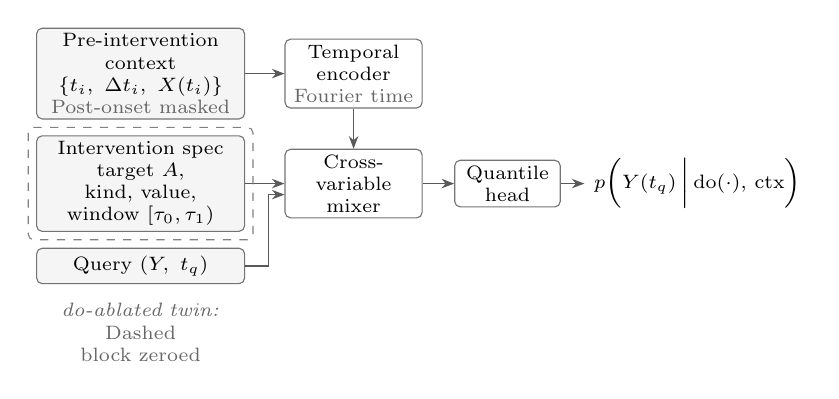
\begin{tikzpicture}[
      font=\scriptsize,
      box/.style={draw=black!55, rounded corners=2pt, align=center,
                  minimum height=4.5mm, inner sep=2pt},
      dim/.style={box, fill=black!4},
      arr/.style={-{Stealth[length=1.6mm]}, black!65},
      node distance=2mm and 3.5mm
    ]
    \node[dim, text width=25mm] (ctx)
      {Pre-intervention context\\ $\{t_i,\ \Delta t_i,\ X(t_i)\}$\\ \textcolor{black!60}{Post-onset masked}};
    \node[dim, text width=25mm, below=of ctx] (spec)
      {Intervention spec\\ target $A$, kind, value,\\ window $[\tau_0, \tau_1)$};
    \node[dim, text width=25mm, below=of spec] (query)
      {Query $(Y,\ t_q)$};
    \node[box, right=5mm of ctx, text width=16mm] (enc)
      {Temporal encoder\\ \textcolor{black!60}{Fourier time}};
    \node[box, text width=16mm] (mix) at (enc |- spec) {Cross-variable\\ mixer};
    \node[box, right=4mm of mix, text width=12mm] (head)
      {Quantile\\ head};
    \node[right=3mm of head, align=center] (out)
      {$p\big(Y(t_q)\,\big|\,\dodo{\cdot},\,\mathrm{ctx}\big)$};
    \draw[arr] (ctx) -- (enc);
    \draw[arr] (enc.south) -- (mix.north);
    \draw[arr] (spec) -- (mix);
    \draw[arr] (query.east) -| ([xshift=-2mm]mix.south west) |- ([yshift=-1.4mm]mix.west);
    \draw[arr] (mix) -- (head);
    \draw[arr] (head) -- (out);
    \draw[black!50, dashed, rounded corners=2pt]
      ([xshift=-1mm,yshift=1mm]spec.north west) rectangle ([xshift=1mm,yshift=-1mm]spec.south east);
    \node[anchor=north, black!60, text width=25mm, align=center] at ([yshift=-1.2mm]query.south)
      {\emph{do-ablated twin:}\\ Dashed block zeroed};
  \end{tikzpicture}
\end{document}
